\chapter{Job scheduling}
\label{chap:refs}

Job scheduling allocates jobs to machines. There are many different variants of job scheduling, each with different constraints and assumptions. This thesis deals with three particular variants: JSSP, FJSP, and DJSP. This chapter defines each variant and discusses relevant graph representations and Markov Decision Process (MDP) formulations.

\section{Job-Shop Scheduling Problem}

The simplest variant of job scheduling called JSSP consists of a set of jobs $\mathcal{J}$ and a set of machines $\mathcal{M}$ \cite{YamadaNakanoJSSP}. Each job has an associated ordered sequence of non-overlapping operations $O_{ij}$ to be processed. Operation $\mathcal{O}_{ij}$ represents uninterrupted processing of job $J_i \in \mathcal{J}$ on machine $M_j \in \mathcal{M}$ with processing time $p_{ij}$. Each machine can process only one operation at a time. A schedule is a set of start times $S_{ij}$ for each operation $O_{ij}$ that satisfies these constraints. Completion times $C_{ij} = S_{ij} + p_{ij}$ denote the end of each operation. The JSSP solution is a schedule minimizing total makespan $C_\text{max} = \text{max}_{i,j} \{C_{ij}\}$ \cite{zhang2020learning}. An example of a JSSP instance with three jobs and three machines (3x3) is shown in table 1.1 \cite{YamadaNakanoJSSP}.
\begin{table}[htbp]
    Table 1.1: 3x3 example JSSP instance \cite{YamadaNakanoJSSP}\\
    \vspace{1mm}
    \begin{tabular}{cccc}
    \hline
    job & \multicolumn{3}{c}{Machine (processing time)} \\ \hline
    1   & 1 (3)             & 2 (3)             & 3 (3)            \\
    2   & 1 (2)             & 3 (3)             & 2 (4)            \\
    3   & 2 (3)             & 1 (2)             & 3 (1)            \\ \hline
    \end{tabular}
\end{table}\\
The Gantt-Chart is a convenient tool for visualizing schedules \cite{WILSON2003430}. An example of a solution for the 3x3 problem from Table 1.1 is shown in Figure 1.1.
\begin{center}
    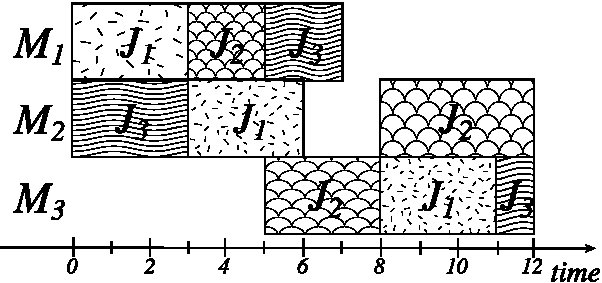
\includegraphics[width=0.8\linewidth]{images/gantt-charrt.pdf}\\
    Figure 1.1: Gantt-Chart of a solution for a 3x3 problem in table 1.1, reproduced from \cite{YamadaNakanoJSSP}
\end{center}

\subsection{JSSP as a disjunctive graph} \label{JSSP as a disjunctive graph}

JSSP can be represented by a disjunctive graph \cite{YamadaNakanoJSSP, BLAZEWICZ2000317} $G = ( V, A \cup E )$, where $V$ denotes a set of vertices corresponding to different operations $O_{ij}$ together with \textit{source} node and \textit{sink} node representing start and end of the schedule, respectively. The source node can be interpreted as a dummy operation preceding all other operations, and the sink node as a dummy operation succeeding all other operations. Both dummy operations have a processing time equal to zero. Nodes $V$ are weighted by the processing time of their corresponding operation. $A$ is a set of conjunctive arcs representing precedence constraints between operations, and between the jobs and dummy operations. $E = \bigcup_{k} E_k$ is a set of disjunctive edges, where $E_k$ is a clique connecting operations that require the same machine $M_k$ for their execution.
\begin{center}
    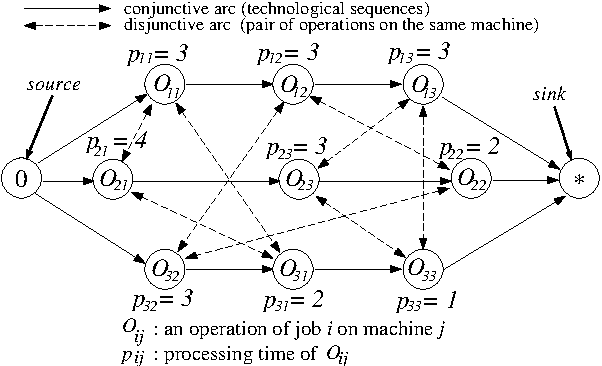
\includegraphics[width=0.75\linewidth]{images/jssp_disjunctive_graph.pdf}\\
    Figure 1.2: Disjunctive graph representation of 3x3 instance in table 1.1, retrieved from \cite{YamadaNakanoJSSP}
\end{center}

Finding a solution to the job-shop scheduling problem can be viewed as defining the ordering between operations requiring the same machine. In the disjunctive graph, this is done by turning all disjunctive arcs into conjunctive arcs \cite{YamadaNakanoJSSP, BLAZEWICZ2000317} in such a way that the resulting graph is a direct acyclic graph (DAG) \cite{doi:10.1287/opre.17.6.941}. The makespan $C_\text{max}$ is then given by the longest weighted path from source to sink.

\subsection{JSSP as a Machine-Operation Graph}

Alternative graph representation proposed in \cite{10226873} represents JSSP as a graph $G = (V, E)$, where $V$ is a set of nodes and $E$ is a set of edges. 
\par
Each node can be either a machine node corresponding to machine $M_j \in \mathcal{M}$ or an operation node corresponding to operation $O_{ij} \in \mathcal{O}$. Features of machine nodes include the status of the corresponding machine and the remaining time of the operation being processed. Features of operation nodes include the status of the operation, the processing time, the remaining time of the operation, and the number of remaining operations in the current job.
\par
Each edge can be either operation-to-operation ($O-O$) edge, machine-to-machine ($M-M$) edge, or operation-to-machine ($O-M$) edge. $O-O$ edges fully connect all operations in the same job, and all machines are fully connected via $M-M$ edges. $O-M$ edge connects operations with machines on which they can be processed.

\section{Flexible Job-shop Scheduling Problem}

FJSP is an extended version of JSSP with the only difference being that each operation $O_{ij} \in \mathcal{O}$ can be processed on any machine $M_k$ from the given subset of machines $\mathcal{M}_{ij} \subseteq \mathcal{M}$ with processing time $p_{ijk}$ \cite{9826438}. Solving FJSP then consists of selecting the appropriate machine for each operation (machine selection) and determining its start time (operation sequencing) \cite{https://doi.org/10.1049/iet-cim.2018.0009}. 

\subsection{Disjunctive graph for FJSP}

Similarly, as in \ref{JSSP as a disjunctive graph}, the disjunctive graph representation for the FJSP can be written as $G = (O, A, E)$ \cite{Brandimarte_1993, 9826438, LEI2022117796}, where $V$ is a set of nodes representing operations and two dummy operations representing start and end, $A$ is a set of conjunctive arcs representing precedence constraints between operations, and $E = \bigcup_{k} E_k$ is a set of disjunctive edges. The only difference with respect to JSSP is that each operation can be part of multiple cliques. An example of disjunctive graph representation for FJSP is shown in figure 1.3.
\begin{center}
    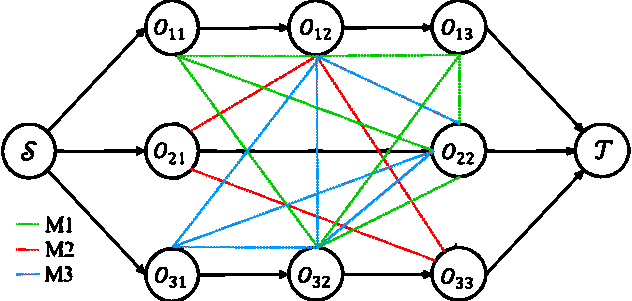
\includegraphics[width=0.75\linewidth]{images/fjsp_disjunctive_graph.pdf}\\
    Figure 1.3: Disjunctive graph representation of FJSP, reproduced from \cite{LEI2022117796}
\end{center}
